\section{Results}
\label{sec:results}

\subsection{Fixed velocity-distribution shape}
\label{sec:fixedshape}

We first fit a single MLR surface to all 14\,876 systems with the shape of the
normal component fixed at its orbital-population reference,
$(B,u_c,C)=(2.544\times10^{-3},35.67,3.1)$, and only $f_{\rm out}$ free
(Fig.~\ref{fig:fixedshape}).  The fit is well converged (maximum
rank-normalised $\widehat R=1.003$, minimum bulk and tail effective sample
sizes $>4\,700$, no divergences).  The inferred MLR is not a small
correction to PARSEC: at $M_G\approx8$ the dynamical masses exceed PARSEC by
$\approx30$\% at all metallicities, for example $0.901^{+0.018}_{-0.017}$
versus $0.696~\msun$ at $M_G=7$ and $\mh=0$.  The excess is confined to
$5\lesssim M_G\lesssim11$; it vanishes at the solar anchor and changes sign
for the faintest stars.  The outlier fraction is
$f_{\rm out}=0.207\pm0.006$.

Figure~\ref{fig:fixedshape} also shows a variant in which the outlier
component is defined on $\tilde u$, that is, it scales with the photometric
mass like the normal component.  This variant raises the mass excess to
$\approx38$--$47$\% and lowers $f_{\rm out}$ to $0.149\pm0.005$: when the
outlier distribution scales with the mass, the outlier term no longer
penalises a larger mass scale, and high-velocity systems are absorbed by the
normal component.  Defining the
outlier component in the observed frame, Eq.~(\ref{eq:out}), removes this
coupling, and we adopt it throughout.  The remaining $\approx30$\% excess is
large compared with the few-per-cent precision of empirical MLRs of nearby
M dwarfs \citep{Mann2019}, and it has the shape of
a mass-scale distortion that peaks where the sample is densest.  This
indicates that the fixed $p_{\rm N}(\tilde u)$ does not describe the observed
velocity distribution, and that the MLR absorbs the mismatch.

\begin{figure*}
\centering
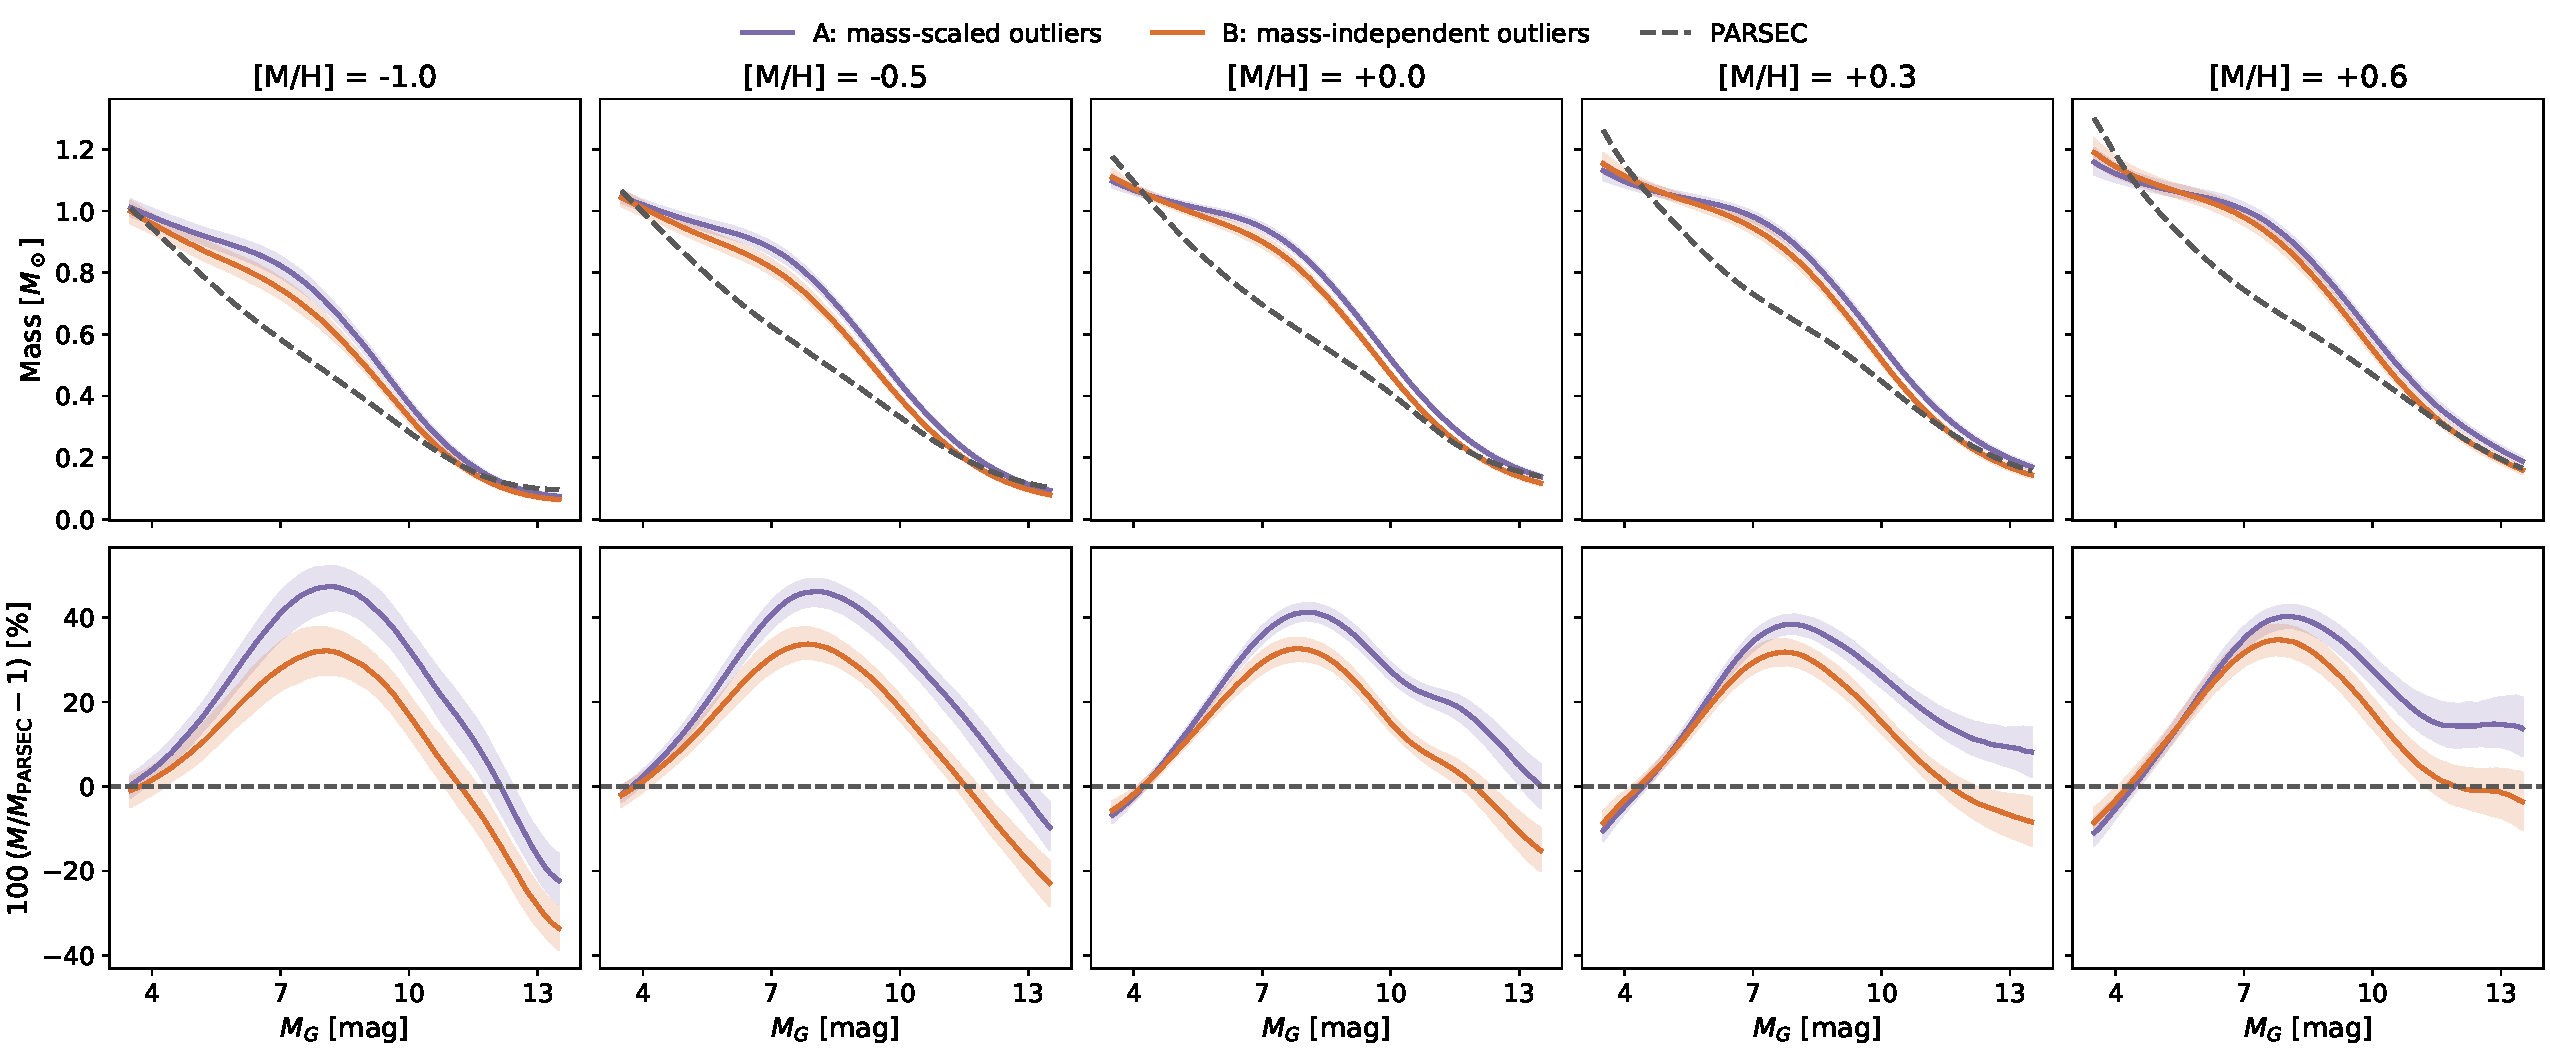
\includegraphics[width=\textwidth]{figures/fixed_shape_residuals.pdf}
\caption{MLR inferred with the velocity-distribution shape fixed to its
orbital-population reference, for the full sample.  Top: mass as a function
of $M_G$ at five metallicities; bottom: relative difference from PARSEC.
Orange: outlier component defined on the observed $u$
(Eq.~\ref{eq:out}); purple: outlier component that scales with the
photometric mass.  Dashed lines show PARSEC; bands are 16--84\% posterior
intervals.}
\label{fig:fixedshape}
\end{figure*}

\subsection{Joint MLR and velocity-distribution fits in metallicity bins}
\label{sec:binresults}

Figure~\ref{fig:bins} and Table~\ref{tab:residuals} present the MLR when the
shape parameters are sampled jointly with the MLR in four independent
metallicity bins.  Freeing the shape removes most of the mass excess of
Sect.~\ref{sec:fixedshape}: in every bin the inferred masses lie within
$\approx15$\% of PARSEC for $M_G\le11$.  The two independent runs per bin
agree to better than 0.25\% in the median mass at every magnitude.

The residuals relative to PARSEC depend systematically on metallicity.  In the
most metal-rich bin ($\mh=0.3$--$0.6$, evaluated at $+0.45$) the stars are
more massive than PARSEC by $8$--$14$\% over $5\le M_G\le13$, and the excess
differs from zero by more than $1\sigma$ everywhere in this range.  In the
most metal-poor bin ($-1.0$ to $-0.5$, at $-0.75$) the masses lie
$3$--$6$\% below PARSEC for $M_G\le11$ and $20$\% below at $M_G=13$.  The two
near-solar bins, which contain 96\% of the sample, agree with PARSEC to
within $\approx7$\% for $M_G\le9$ and fall below it by $10$--$18$\% at
$M_G=13$.  In the $[0,0.3)$ bin the residual changes from $+7$\% at $M_G=7$
to $-13$\% at $M_G=11$, a stronger magnitude dependence than in any other
bin.

\begin{figure}
\centering
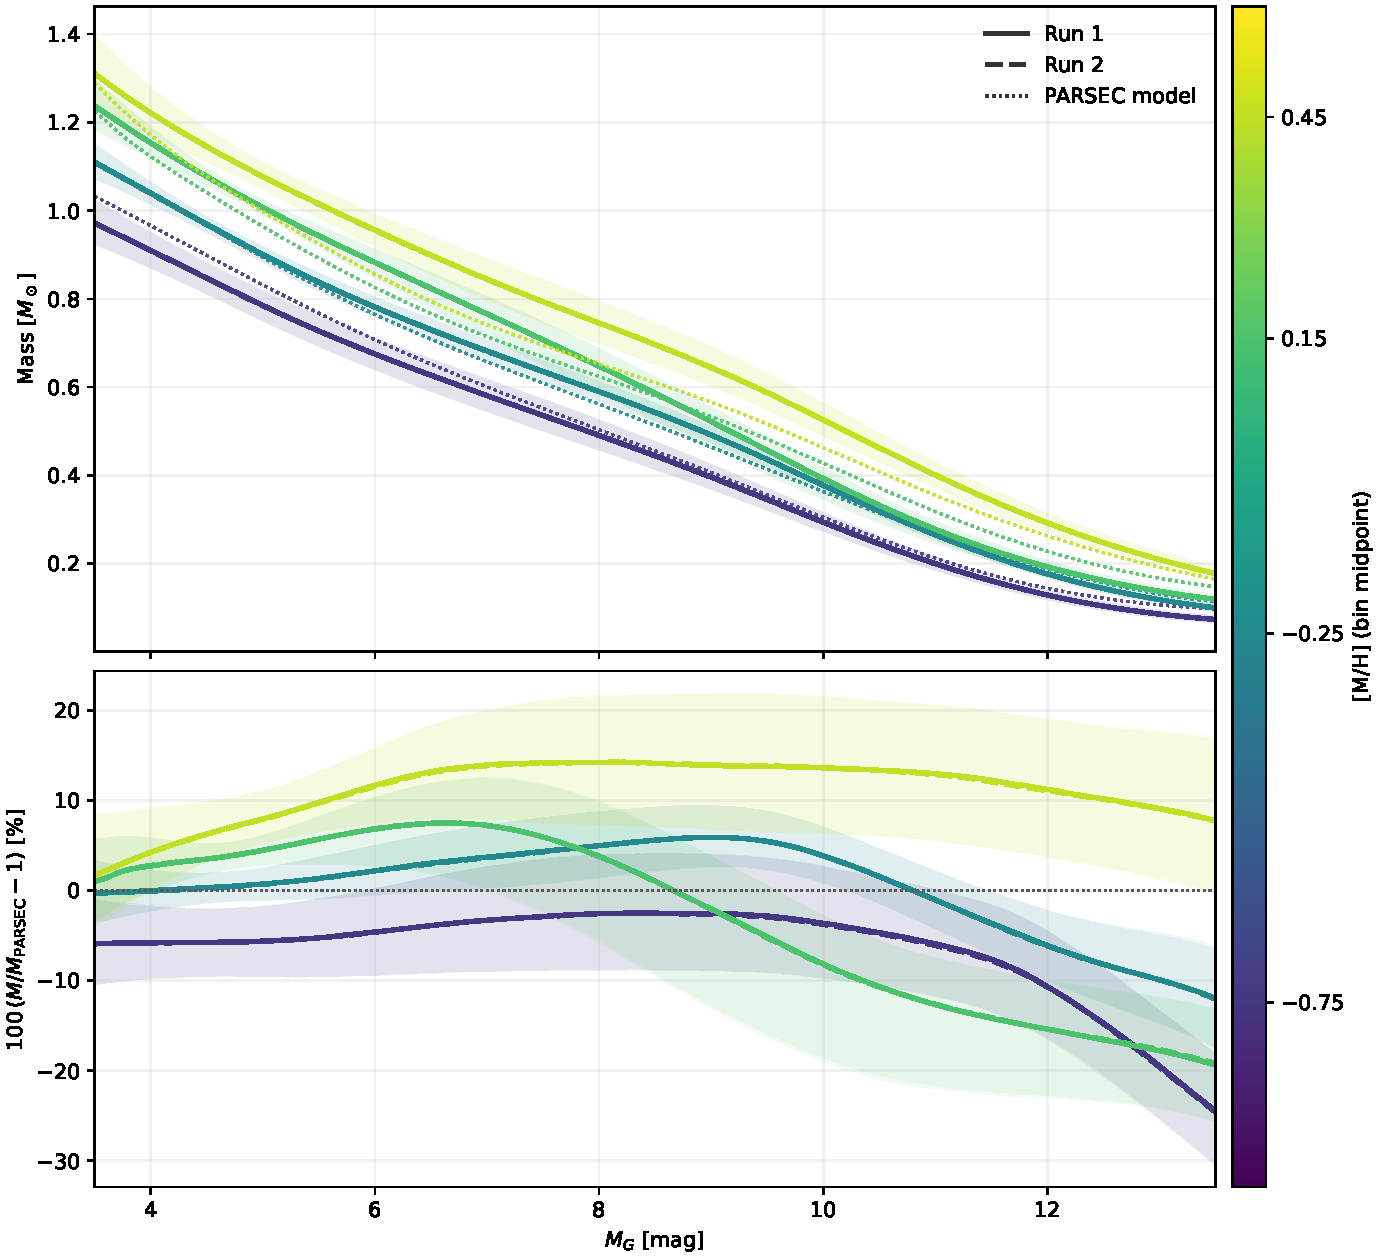
\includegraphics[width=\columnwidth]{figures/mlr_bins_by_mh.pdf}
\caption{MLR from the joint fits of the MLR and velocity-distribution shape
in four independent metallicity bins, evaluated at the bin midpoints
(colour).  Top: posterior median mass (solid and dashed: two independent
runs) and PARSEC (dotted).  Bottom: relative difference from PARSEC.  Bands
are pointwise 16--84\% intervals.}
\label{fig:bins}
\end{figure}

\begin{table*}
\caption{Dynamical mass relative to PARSEC, $100\,(M/M_{\rm P}-1)$, in
per cent.}
\label{tab:residuals}
\centering
\begin{tabular}{@{}lrcccccc@{}}
\toprule
Bin & $N$ & $\mh_{\rm eval}$ & $M_G=5$ & $7$ & $9$ & $11$ & $13$ \\
\midrule
$[-1.0,-0.5)$ & 186 & $-0.75$ &
 $-5.6^{+3.7}_{-3.9}$ & $-3.3^{+5.8}_{-5.6}$ & $-2.5^{+6.4}_{-6.2}$ &
 $-5.9^{+5.9}_{-5.7}$ & $-19.5^{+6.0}_{-5.6}$ \\
$[-0.5,0.0)$ & 9\,618 & $-0.25$ &
 $+0.7^{+1.7}_{-1.6}$ & $+3.7^{+3.4}_{-3.3}$ & $+5.9^{+3.4}_{-3.1}$ &
 $-1.0^{+3.0}_{-3.2}$ & $-9.9^{+5.1}_{-4.8}$ \\
$[0.0,0.3)$ & 4\,687 & $+0.15$ &
 $+4.5^{+1.5}_{-1.6}$ & $+7.2^{+5.2}_{-7.0}$ & $-2.0^{+5.7}_{-10.9}$ &
 $-12.7^{+5.1}_{-9.2}$ & $-17.8^{+5.9}_{-6.3}$ \\
$[0.3,0.6]$ & 385 & $+0.45$ &
 $+7.9^{+3.1}_{-2.6}$ & $+13.9^{+5.9}_{-5.8}$ & $+13.9^{+7.7}_{-7.0}$ &
 $+13.0^{+7.5}_{-7.4}$ & $+9.1^{+8.3}_{-7.6}$ \\
\bottomrule
\end{tabular}
\tablefoot{Posterior medians with 16th and 84th percentiles from the first
run of each bin, evaluated at the bin midpoint $\mh_{\rm eval}$.  The
corresponding PARSEC masses at $M_G=7$ are 0.600, 0.657, 0.714, and
0.741~$\msun$.}
\end{table*}

\subsection{Metallicity dependence of the MLR}
\label{sec:slope}

Because the four bins are fitted independently, the difference between the
two outer bins provides a dynamical measurement of the metallicity
sensitivity of the MLR.  Between $\mh=-0.75$ and $+0.45$ we find
$\dd\ln M/\dd\mh=0.27\pm0.04$ at $M_G=5$, $0.31\pm0.07$ at $M_G=7$,
$0.41\pm0.08$ at $M_G=9$, $0.58\pm0.08$ at $M_G=11$, and $0.75\pm0.09$ at
$M_G=13$ (Table~\ref{tab:slope}).  The sign agrees with stellar-evolution
theory, and the sensitivity increases towards fainter stars, as in PARSEC.
The amplitude, however, is $1.4$--$1.8$ times the PARSEC value at every
magnitude.  Across the 1.2~dex between the outer bins, the mass at fixed
$M_G$ thus increases by 37\% at $M_G=5$ and by a factor of 2.4 at
$M_G=13$, compared with 20\% and a factor of 1.8 in PARSEC.

\begin{table}
\caption{Metallicity sensitivity of the MLR between the outer bins.}
\label{tab:slope}
\centering
\begin{tabular}{@{}cccc@{}}
\toprule
$M_G$ & $\dd\ln M/\dd\mh$ & PARSEC & Ratio \\
\midrule
5  & $0.265^{+0.041}_{-0.039}$ & 0.152 & 1.74 \\
7  & $0.311^{+0.067}_{-0.065}$ & 0.176 & 1.77 \\
9  & $0.406^{+0.076}_{-0.074}$ & 0.276 & 1.47 \\
11 & $0.580^{+0.075}_{-0.074}$ & 0.428 & 1.36 \\
13 & $0.746^{+0.086}_{-0.085}$ & 0.493 & 1.52 \\
\bottomrule
\end{tabular}
\tablefoot{Finite difference of $\ln M$ between $\mh=+0.45$ and $-0.75$,
divided by 1.2~dex, from independent posterior draws of the two bins.}
\end{table}

\subsection{Velocity-distribution shape and outlier fraction}
\label{sec:shape}

Table~\ref{tab:shape} lists the posteriors of the shape parameters and of
$f_{\rm out}$.  All bins prefer a smaller $B$ and $u_c$ than the
orbital-population reference: $u_c\approx28$--$30$ in the three bins with
$\mh>-0.5$, compared with 35.67, and $B$ within 35\% of the lower edge of the
prior box.  In the $[-0.5,0)$ bin, which holds 65\% of the sample,
$B=0.716^{+0.025}_{-0.012}\times10^{-3}$ and $C=2.69^{+0.28}_{-0.14}$ lie
against the lower limits $B=0.7\times10^{-3}$ and $C=2.5$ of the explored
range.  A smaller $u_c$ moves the exponential cut-off of
Eq.~(\ref{eq:good}) to lower $\tilde u$, so that a given observed $u$
requires a larger $\sqrt{M_{\rm tot}}$; this is the direction that allows the
MLR to return towards PARSEC.  The metal-poor bin is the exception, with
$u_c=39.6^{+2.8}_{-3.4}$, above the reference value.

The outlier fraction is $0.17$--$0.23$ in the three bins with $\mh<0.3$
and $0.107^{+0.025}_{-0.022}$ in the metal-rich bin.

\begin{table}
\caption{Velocity-distribution shape and outlier fraction.}
\label{tab:shape}
\centering
\small
\setlength{\tabcolsep}{4pt}
\begin{tabular}{@{}lcccc@{}}
\toprule
Bin & $10^3B$ & $u_c$ & $C$ & $f_{\rm out}$ \\
\midrule
$[-1.0,-0.5)$ & $0.90^{+0.26}_{-0.14}$ & $39.6^{+2.8}_{-3.4}$ &
 $5.2^{+4.0}_{-2.0}$ & $0.173^{+0.051}_{-0.044}$ \\
$[-0.5,0.0)$ & $0.716^{+0.025}_{-0.012}$ & $29.3^{+0.4}_{-0.4}$ &
 $2.69^{+0.28}_{-0.14}$ & $0.230^{+0.007}_{-0.007}$ \\
$[0.0,0.3)$ & $0.74^{+0.08}_{-0.03}$ & $29.1^{+4.2}_{-0.8}$ &
 $3.8^{+3.7}_{-0.9}$ & $0.188^{+0.014}_{-0.038}$ \\
$[0.3,0.6]$ & $0.93^{+0.39}_{-0.18}$ & $27.8^{+1.9}_{-1.6}$ &
 $3.6^{+1.8}_{-0.8}$ & $0.107^{+0.025}_{-0.022}$ \\
\midrule
Reference & 2.544 & 35.67 & 3.1 & -- \\
Prior range & 0.7--3.3 & 24--44 & 2.5--13.5 & Beta$(3,12)$ \\
\bottomrule
\end{tabular}
\tablefoot{Posterior medians and 16--84\% intervals from the first run of
each bin.}
\end{table}

\subsection{Sampling diagnostics}

Table~\ref{tab:diagnostics} summarises the convergence of the eight
Stage-2 runs.  Six runs have $\widehat R<1.003$ and minimum effective sample
sizes above 1\,900.  The two runs of the $[0.0,0.3)$ bin mix more slowly
(minimum ESS 213 and 137, maximum $\widehat R=1.007$ and 1.026); their medians
agree to 0.25\%, but their intervals, which are broad and asymmetric in
Tables~\ref{tab:residuals} and \ref{tab:shape}, should be regarded as
provisional.

\begin{table}
\caption{Convergence diagnostics of the Stage-2 runs.}
\label{tab:diagnostics}
\centering
\small
\begin{tabular}{@{}lcccc@{}}
\toprule
 & \multicolumn{2}{c}{Run 1} & \multicolumn{2}{c}{Run 2} \\
Bin & max $\widehat R$ & min ESS & max $\widehat R$ & min ESS \\
\midrule
$[-1.0,-0.5)$ & 1.0020 & 2620 & 1.0014 & 3139 \\
$[-0.5,0.0)$  & 1.0024 & 2079 & 1.0009 & 1922 \\
$[0.0,0.3)$   & 1.0067 & 213  & 1.0255 & 137 \\
$[0.3,0.6]$   & 1.0015 & 2247 & 1.0021 & 2258 \\
\bottomrule
\end{tabular}
\tablefoot{Four chains of 2\,000 retained draws per run; no divergent
transitions in any run.}
\end{table}
